\documentclass[12pt, a4paper, onecolumn, oneside, final]{report}
\usepackage[utf8]{inputenc}
%\usepackage{fontspec}
%\setmainfont{Times New Roman}
%%%%
\usepackage{tocbibind} %%% untuk memasukkan bibliography pada daftar isi
%
%%%%%%  adding image %%%
\usepackage{graphicx}
\graphicspath{{images/}}
\newcommand{\pic}{Gambar}
%%%%
\usepackage{setspace} % pengaturan line spacing 
%%%%%% 
\usepackage[paper=a4paper,headheight=0pt,left=4cm,top=4cm,right=3cm,bottom=3cm]{geometry}
\usepackage[font=footnotesize,format=plain,labelfont=bf,up,textfont=up]{caption} 
\captionsetup{labelsep=space}
\usepackage{amsmath}
\usepackage{amsfonts}
\usepackage{bm}
%%%%% For Markdown Support
\usepackage{markdown}
%%%%% Coding utils
\usepackage{forest}
\usepackage{listings}
\usepackage{xcolor}
%%%%% listing style
\definecolor{codegreen}{rgb}{0,0.6,0}
\definecolor{codegray}{rgb}{0.5,0.5,0.5}
\definecolor{codepurple}{rgb}{0.58,0,0.82}
\definecolor{backcolour}{rgb}{0.95,0.95,0.92}

\lstdefinestyle{mystyle}{
    backgroundcolor=\color{backcolour},   
    commentstyle=\color{codegreen},
    keywordstyle=\color{magenta},
    numberstyle=\tiny\color{codegray},
    stringstyle=\color{codepurple},
    basicstyle=\ttfamily\footnotesize,
    breakatwhitespace=false,         
    breaklines=true,                 
    captionpos=b,                    
    keepspaces=true,                 
    numbers=left,                    
    numbersep=5pt,                  
    showspaces=false,                
    showstringspaces=false,
    showtabs=false,                  
    tabsize=2
}

\lstset{style=mystyle}

%define Javascript language
\lstdefinelanguage{JavaScript}{
keywords={typeof, new, true, false, catch, function, return, null, catch, switch, var, if, in, while, do, else, case, break},
keywordstyle=\color{blue}\bfseries,
ndkeywords={class, export, boolean, throw, implements, import, this},
ndkeywordstyle=\color{darkgray}\bfseries,
identifierstyle=\color{black},
sensitive=false,
comment=[l]{//},
morecomment=[s]{/*}{*/},
commentstyle=\color{purple}\ttfamily,
stringstyle=\color{red}\ttfamily,
morestring=[b]',
morestring=[b]"
}

%define json
\colorlet{punct}{red!60!black}
\definecolor{background}{HTML}{EEEEEE}
\definecolor{delim}{RGB}{20,105,176}
\colorlet{numb}{magenta!60!black}

\lstdefinelanguage{json}{
    basicstyle=\normalfont\ttfamily,
    numbers=left,
    numberstyle=\scriptsize,
    stepnumber=1,
    numbersep=8pt,
    showstringspaces=false,
    breaklines=true,
    frame=lines,
    backgroundcolor=\color{background},
    literate=
     *{0}{{{\color{numb}0}}}{1}
      {1}{{{\color{numb}1}}}{1}
      {2}{{{\color{numb}2}}}{1}
      {3}{{{\color{numb}3}}}{1}
      {4}{{{\color{numb}4}}}{1}
      {5}{{{\color{numb}5}}}{1}
      {6}{{{\color{numb}6}}}{1}
      {7}{{{\color{numb}7}}}{1}
      {8}{{{\color{numb}8}}}{1}
      {9}{{{\color{numb}9}}}{1}
      {:}{{{\color{punct}{:}}}}{1}
      {,}{{{\color{punct}{,}}}}{1}
      {\{}{{{\color{delim}{\{}}}}{1}
      {\}}{{{\color{delim}{\}}}}}{1}
      {[}{{{\color{delim}{[}}}}{1}
      {]}{{{\color{delim}{]}}}}{1},
}
 
%%%%%
\usepackage{pslatex} % untuk menggunakan font times new roman
%%%%%%
\usepackage{fancyhdr}
%%%%%%% Pengaturan header dan footer dalam dokumen.
\fancyhf{} 
\fancyhead[R]{\thepage}
\renewcommand{\headrulewidth}{0.0pt}
\pagestyle{fancy}
\setlength{\headheight}{14pt}
\addtolength{\topmargin}{-2pt}
%%%%%%%% pengaturan tabel dan gambar
\usepackage{float}
  \floatplacement{figure}{H}
  \floatplacement{table}{H}
%%%%%%%%  
\usepackage{pdfpages} %% untuk memasukkan pdf pada dokumen 
%%%%%%% Konfigurasi Daftar Pustaka
\usepackage{natbib}
\setcitestyle{citesep={;}, aysep={,}} % tambah semikolon dan koma di sitasi
\renewcommand\harvardyearleft{ \unskip } % remove parantheses di dapus
\renewcommand\harvardyearright[1]{.} % remove parantheses di dapus
%%%%%
\usepackage[bahasai]{babel} % Paket bahasa indonesia dan inggris
%%%%%%
%%%%%% konfigurasi setiap subbab
\usepackage{titlesec}
\titleformat{\section}
  {\normalfont\fontsize{12}{12}\bfseries}
  {\thesection}
  {1em}
  {} 
\titleformat{\subsection}
  {\normalfont\fontsize{12}{12}\bfseries}
  {\thesubsection}
  {1em}
  {} 
%%%%%%% Konfigurasi untuk tajuk bab %%%%%%%%%%%%%%%%%%%%%%%%%%%%%%%%%%%%%%%%%%
\makeatletter
\def\@makechapterhead#1{%
  %%%%\vspace*{50\p@}% %%% removed! % <----------------- Space from top of page to Chapter #
  {\parindent \z@ \centering \normalfont
    \ifnum \c@secnumdepth >\m@ne
        \large\bfseries \MakeUppercase{\@chapapp}\space \thechapter % <--- uppercase
        \par\nobreak
        \vskip 5\p@ %<-------------- Space between Chapter # and title
    \fi
    \interlinepenalty\@M
    \large \bfseries #1\par\nobreak
    \vskip 30\p@
  }}
%
\def\@makeschapterhead#1{% % format tulisan "daftar isi" 
  %%%%%\vspace*{50\p@}% %%% removed! % <----------------- Space from top of page to Chapter #
  {\parindent \z@ \centering
    \normalfont
    \interlinepenalty\@M
    \large\bfseries \MakeUppercase  #1\par\nobreak
    \vskip 30\p@
 }}
\makeatother
%%%%%%%%%%%%%%%%%%%%%%%%%%%%%%%%%%%%%%%%%%%%%%%%%%%%%%%%%%%%%%%%%%%%%%%%%%%%%
\usepackage{indentfirst} % Indentasi paragraf pertama
\setlength{\parindent}{1.2cm}
%%%%%%%%%%%%%%%%%%%%%%%%Paket untuk menggambar senyawa kimia%%%%
\usepackage{chemfig}
\usepackage[version=4]{mhchem}
\usepackage{chemnum}
\makeatletter
\def\Hv@scale{0.65}
\makeatother
\DeclareMathAlphabet{\foo}{OT1}{phv}{m}{n}
\renewcommand*\printatom[1]{\ensuremath{\foo{#1}}}
\makeatother
\setchemfig{double bond sep = 0.20700 em,  % 'Bond Spacing' 
            fixed length = false,    % 'Fixed Length'
            bond offset = 0.18265 em, % 'Margin Width'
            bond style={line width=0.50pt},
            atom sep = 1.2 em}
%%%%%%%%%%%%%%%%%%%%%%%%%%%%%%%%%%%%%%%%%%%%%%%%%%%%%%%
\usepackage[hidelinks]{hyperref}
%%%%%Table of Contents typography%%%%%%%%%%%%%%%%%%%%%%
\usepackage[titles]{tocloft}
\newlength\mylength
\renewcommand\cftchappresnum{\chaptername~}
\settowidth\mylength{\cftchappresnum\cftchapaftersnum\quad}
\addtolength\cftchapnumwidth{2.3em}
%%%%%%%%%%%%%%%%%%%%%%%%%%%%Paket untuk pengaturan tabel%%%%%%%%%%
\usepackage{booktabs}
\usepackage{multirow}
\usepackage{colortbl}
%%%%%%%%%%%%%%%%%%%%%%%%%%%%Paket untuk penulisan Satuan Internasional%%%
\usepackage{siunitx}
\DeclareSIUnit{\Molar}{M}
\DeclareSIUnit{\calorie}{cal}
\DeclareSIUnit{\Calorie}{\kilo\calorie}
%%%%%%%%%%%%%%%%%%%%%%%%%%%%%%%%%%%%%%%%%%%%%%%%%%%%%
%%%%%%%%%%-----KONTEN PENELITIAN-----%%%%%%%%%%%%%%%%%%%%%%%%%%%%%%%%%%%%%%%%
\begin{document}

\singlespacing
\begin{titlepage}
    \begin{center}
        
        \Large
        \textbf{LAPORAN AKHIR} \\
        \textbf{MAGANG \& STUDI INDEPENDEN BERSERTIFIKAT} \\
        \textbf{CLOUD COMPUTING PATH} \\
        \textbf{di Bangkit Academy 2022 by Google, GoTo, Traveloka} \\
        \textbf{PT Presentologics} \\

        
        \vfill
        
        Diajukan untuk memenuhi persyaratan kelulusan \\
        Program MSIB MBKM
        
        \vfill
        
        %%% Jika tesis uncomment line untuk tesis dan comment line untuk disertasi %%%%%
        \large
        %\textbf{TESIS} \\
        %\small
        %\textbf{Untuk memenuhi salah satu syarat ujian \\
        %Guna memperoleh gelar Magister Kimia\\
        %Program Pendidikan Magister Program Studi Kimia  \\
        %Konsentrasi...}

        \vfill
        
        \large
 
        
        \begin{center}
            oleh: \\
            I Putu Cahya Adi Ganesha / 52419866
        \end{center}
        
        \vfill
        
        
\includegraphics[width=4.0cm]{front/Logo-Gunadarma-Vector-Universitas-Gunadarma.jpg}
        
        \large
        \textbf{TEKNIK INFORMATIKA UNIVERSITAS GUNADARMA} \\
        \textbf{2022}
        
    \end{center}
\end{titlepage}

\pagenumbering{roman} %Gunakan penomoran romawi

\setcounter{page}{1}
\singlespacing

\chapter*{LEMBAR PENGESAHAN TEKNIK INFORMATIKA UNIVERSITAS GUNADARMA}
{\setstretch{1.5}
\vspace*{0.5cm}
\begin{center}
    \textbf{STUDI INDEPENDEN BERSERTIFIKAT CLOUD COMPUTING LEARNING PATH} \\
    \textbf{di Bangkit Academy 2022 by Google, GoTo, Traveloka} \\
    \textbf{PT Presentologics} 
    
\end{center}

\vspace*{0.5cm}

\begin{center}
    oleh: \\
    I Putu Cahya Adi Ganesha / 52419866
\end{center}

\vfill

\begin{center}
    disetujui dan disahkan sebagai \\
    Laporan Studi Independen Bersertifikat Kampus Merdeka \\
\end{center}

\vspace{2mm}

\vspace*{0.2cm}

\vspace{5mm}

\vfill
\noindent Depok, 20 Juli \\
\noindent Pembimbing Studi Independen Teknik Informatika Universitas Gunadarma \\

\vspace{2.3cm}

\noindent \underline{Hurnaningsih, S.Kom., MM.} \\
\noindent NIP:

\vspace{10mm}


\vspace*{0.5cm}
}




\addcontentsline{toc}{chapter}{Lembar Pengesahan Prodi \& Universitas}

\chapter*{LEMBAR PENGESAHAN}
{\setstretch{1.5}
\vspace*{0.5cm}
\begin{center}
    \textbf{STUDI INDEPENDEN BERSERTIFIKAT CLOUD COMPUTING LEARNING PATH} \\
    \textbf{di Bangkit Academy 2022 by Google, GoTo, Traveloka} \\
    \textbf{PT Presentologics} 
    
\end{center}

\vspace*{0.5cm}

\begin{center}
    oleh: \\
    I Putu Cahya Adi Ganesha / 52419866
\end{center}

\vfill

\begin{center}
    disetujui dan disahkan sebagai \\
    Laporan Studi Independen Bersertifikat Kampus Merdeka \\
\end{center}

\vspace{2mm}

\vspace*{0.2cm}

\vspace{5mm}

\vfill
\noindent Bandung, 17 Juli 2022 \\
\noindent Learning Support Manager \\
\noindent Bangkit Academy 2022 \\

\vspace{2.3cm}

\noindent \underline{Adrianus Yoza Aprilio} \\
\noindent ID. 01032015004

\vspace{10mm}


\vspace*{0.5cm}
}
\addcontentsline{toc}{chapter}{Lembar Pengesahan}

\chapter*{ABSTRAK}
\noindent \textbf{Bangkit 2022} merupakan program yang berada di bawah naungan \textbf{Merdeka Belajar Kampus Merdeka}, yang memiliki tujuan sesuai kutipan dari laman web resminya \textit{"Kampus Merdeka merupakan bagian dari kebijakan Merdeka Belajar oleh Kementerian Pendidikan, Kebudayaan, Riset, dan Teknologi Republik Indonesia yang memberikan kesempatan bagi mahasiswa/i untuk mengasah kemampuan sesuai bakat dan minat dengan terjun langsung ke dunia kerja sebagai persiapan karier masa depan."}. Program \textbf{Bangkit 2022} terdiri dari tiga \textit{learning path} yaitu \textit{Android (Mobile Development), Machine Learning, dan Cloud Computing}, dengan laporan ini disesuaikan dengan \textit{path} \textit{Cloud Computing} yang merupakan \textit{leearning path} yang saya ambil, yang dalam eksekusi programnya mempelajari mengenai penggunaan platform \textbf{Google Cloud Platform}, diselingi dengan materi \textit{soft skill}. Dalam pembelajaran, pengimplementasian riil dilakukan dalam proyek \textit{capstone} yaitu \textbf{Safe Route} yang me-\textit{leverage} penggunaan \textit{cloud platform}.

\vspace{5mm}
\addcontentsline{toc}{chapter}{Abstrak}

\chapter*{ABSTRACT}
\noindent \textbf{Bangkit 2022} is a program under the auspices of \textbf{Merdeka Be-
belajar Kampus Merdeka}, which has a purpose according to an excerpt from the website
Officially, \textit{"Independence Campus is part of the Independent Learning policy"
by the Ministry of Education, Culture, Research and Technology of the Republic of Indonesia
who provides an opportunity for students to hone their skills
according to talents and interests by going directly into the world of work as preparation
future career.”} The \textbf{Bangkit 2022} program consists of three learning paths, namely
\textit{Android (Mobile Development), Machine Learning, and Cloud Computing}, with
this report is adapted to the \textbf{Cloud Computing} path which is a learning
the path I took, which in the execution of the program learns about
the use of the \textbf{Google Cloud Platform platform}, interspersed with soft skills material.
In learning, real implementation is carried out in capstone projects
namely \textbf{Safe Route} which leverages the use of cloud platforms.

\vspace{5mm}
\addcontentsline{toc}{chapter}{Abstract}

\chapter*{KATA PENGANTAR}
{\setstretch{1.5}
Ucapan terima kasih saya berikan kepada \textbf{Kementrian Pendidikan, Kebudayaan, Riset dam Teknologi Republik Indonesia} yang telah melalui kebijakan \textit{Merdeka Belajar Kampus Merdeka}, dengan salah satu programnya yaitu \textbf{Bangkit 2022} yang telah memberikan kesempatan yang bisa dibilang cukup langka, yaitu kesempatan untuk mempelajari teknologi terbaru dengan kurikulum yang disesuaikan dengan dunia \textit{professional}. Tidak lupa juga puji syukur kepada Tuhan Yang Maha Esa yang telah memberikan kesempatan tersebut kepada saya, serta ucapan terima kasih terutama kepada:
\begin{enumerate}
    \item Ibu Prof. Dr. E.S. Margianti, SE., MM., selaku Rektor Universitas Gunadarma
    \item Ibu Dr. Lintang Yuniar Banowosari, S.Kom., M.Sc., selaku Ketua Jurusan Teknik
Informatika Universitas Gunadarma.
    \item Ibu Hurnaningsih, S.Kom., MM., selaku dosen pendamping dalam program Bangkit 2022.
    \item Ibu Ike Putri Kusumawijaya, ST., MMSI., selaku dosen pendamping dalam program Bangkit 2022.
    \item Ibu Astie Darmayantie, ST, MMSI, MSc., beserta rekan yang membantu memfasilitasi mahasiswa Gunadarma dalam mendaftar ke dalam program Bangkit 2022.
    \item Seluruh tim Bangkit 2022 beserta jajaran pimpinan, atas usahanya dalam membentuk lingkungan belajar yang menyenangkan dan mendukung perkembangan siswa.
    \item Seluruh mentor yang telah berkontribusi dalam Bangkit 2022.
\end{enumerate}
Tidak lupa juga, ucapan rasa terima kasih terhadap semua yang telah mewujudkan program \textbf{Bangkit 2022} ini yang terlalu banyak untuk disebutkan satu-satu. Semoga ilmu yang didapatkan dengan terlaksananya program ini dapat turut digunakan dalam rangka memajukan bangsa Indonesia, Berikut adalah laporan akhir yang merupakan sebagai media visibilitas dari pengaruh program \textbf{Bangkit 2022} ini.

\vspace{2.3cm}

\begin{flushright}
Karawang, 20 Juli 2022 \\
\vspace{2cm}
I Putu Cahya Adi Ganesha
\end{flushright}
}

\addcontentsline{toc}{chapter}{Kata Pengantar}

\singlespacing
\thispagestyle{plain}
\tableofcontents
\thispagestyle{plain}
\listoffigures
\clearpage

\pagenumbering{arabic} %Gunakan penomoran arab
\doublespacing
\renewcommand{\thechapter}{\Roman{chapter}}
\renewcommand{\thesection}{\arabic{chapter}.\arabic{section}}
\renewcommand{\thefigure}{\arabic{chapter}.\arabic{figure}}
\renewcommand{\thetable}{\arabic{chapter}.\arabic{table}}
\renewcommand{\thelstlisting}{\arabic{lstlisting}}

\chapter{PENDAHULUAN} 
\section{Latar Belakang}

Revolusi digital yang sedang dialami oleh Indonesia, yang salah satu bukti riilnya yaitu gaungan \textit{Revolusi Industri 4.0} yang sering didengar belakangan ini menuntut perkembangan yang sangat besar pada talenta digital Indonesia, yang sayang-nya sampai saat ini sedang mengalami \textit{"krisis talenta digital"}. Krisis tersebut merujuk kurangnya sumber daya manusia profesional yang bergerak pada bidang digital, sedangkan ketersediaan tersebut harus segera dipenuhi karena tuntutan yang turut berkembang secara eksponensial. 

Tiga dari banyak sektor yang memiliki permintaan yang paling banyak adalah \textit{mobile developer}, mengacu kepada penggunaan perangkat \textit{smartphone} dalam kehidupan sehari-hari yang semakin hari semakin banyak penggunanya sehingga menjadikannya \textit{prime market} untuk pengembang, \textit{cloud computing} yang merujuk kepada adopsi besar-besaran \textit{cloud platform} di dunia guna mendukung kebutuhan \textit{developer} maupun perusahaan dari skala kecil ke besar yang dalam penggunaannya sendiri membutuhkan \textit{expertise} tersendiri, dan \textit{machine learning} yang merujuk kepada penggunaan kecerdasan artifisial yang makin sering digunakan untuk mengotomatisasi berbagai tugas sederhana ke komplex sehingga membutuhkan seseorang yang ahli untuk mewujudkan \textit{model} untuk mengimplementasikannya. 

Program \textbf{Bangkit 2022}, merupakan program yang sesuai kutipan dalam laman resminya \textit{"Dirancang untuk mempersiapkan siswa dengan keterampilan yang dibutuhkan dan sertifikasi teknologi, kurikulum Bangkit menawarkan 3 jalur pembelajaran interdisipliner - pembelajaran mesin, pengembangan seluler, dan komputasi awan. Pada akhir program ini, Anda akan dilengkapi dengan keahlian teknologi dan soft skill yang Anda butuhkan untuk berpindah dari dunia akademis ke tempat kerja dan sukses di perusahaan terkemuka."} dan \textit{Tahun ini, Bangkit ditawarkan sebagai program Studi Independen Bersertifikat Kampus Merdeka yang disetujui dan didukung oleh Kementerian Pendidikan dan Kebudayaan Republik Indonesia. Kami mendaftarkan hingga 3.000 mahasiswa di 3 jalur pembelajaran untuk membantu mereka mengembangkan keterampilan yang dibutuhkan di bidang teknologi dan mempersiapkan mereka untuk mengikuti sertifikasi Google.Program ini berlangsung sepanjang semester genap 2022.} Bertujuan sebagai program yang mempersiapkan siswasnya agar \textit{job-ready}, dengan \textit{skill} yang sedang memiliki banyak sekali permintaan, seperti pengembangan \textit{mobile}, \textit{cloud computing}, dan \textit{machine learning}.

\section{Lingkup} \label{lingkup}

Dalam program ini saya berperan sebagai \textit{mentees/cohort} atau siswa \textit{cloud computing} mempelajari mengenai penggunaan \textit{cloud platform Google}, yang perlu melakukan beberapa kegiatan (akan dibahas lebih detail pada bab 2). Dengan fokus berada pada pengimplementasian dari ilmu yang telah didapat dari program ini dituangkan dalam sebuah proyek akhir (\textit{capstone project}), yang menjadi salah satu bahan utama dalam evaluasi peserta \textbf{Bangkit 2022} dalam mengaplikasikan ilmu yang telah didapat ke dalam sebuah produk yang siap diluncurkan dan diikuti dengan tema yang cukup menarik tentunya. Proyek ini menuntut seluruh aspek dari \textit{learning path} terwujud, mulai dari basis proyek yang dilakukan dengan \textit{kotlin} yang dirancang khusus untuk \textit{android}, penambahan \textit{core feature} oleh \textit{machine learning} dan infrastruktur pendukung dari \textit{cloud computing}.

\section{Tujuan}

Dengan mengambil visi dan misi dari program \textbf{Bangkit 2022} ini, tujuan pribadi saya dalam mengikuti program ini tentunya mencari ilmu pengetahuan yang dapat diandalkan serta \textit{up-to-date} dengan \textit{demand} yang dapat ditemukan secara riil pada kehidupan sehari-hari, dalam jangka pelaksanaan program, pembelajaran mengenai \textit{web development} secara fundamental yang terdiri dari \textit{frontend} dan \textit{backend}, diikuti dengan pembelajaran yang berkaitan dengan \textit{cloud} itu sendiri dalam \textbf{Google Cloud Platform}, yang di dalamnya dapat dijabarkan menjadi sub-material seperti jaringan, sistem operasi, \textbf{DevOps}, \textbf{SRE}, basis data dan lain-lain.

Serta dapat mengimplementasikan hal-hal yang telah disebutkan di atas ke dalam sebuah produk jadi yang diharapkan dapat berperan sebagai solusi terhadap masalah yang dialami oleh penduduk di Indonesia. Pada akhirnya deretan acara dalam program mendorong siswanya untuk mempelajari sebuah keahlian yang sedang dalam permintaan, fasih dalam keahlian tersebut agar dalam status yang \textit{work-ready} diikuti dengan \textit{soft-skill} yang akan turut membantu kehidupan para siswanya.

Mendasari pernyataan ini berdasarkan pernyataan yang sudah diberikan sebelumnya pada latar belakang dan lingkup, secara \textit{Long-term} tujuan utama dari pengadaan program ini adalah untuk mengatasi \textit{"krisis talenta digital"}, yang diharapkan dapat mendongkrak perkembangan Indonesia. 

\chapter{LINGKUNGAN ORGANISASI BANGKIT ACADEMY}
\section{Struktur Organisasi}

Bangkit didesain untuk mempersiapkan peserta dengan kecakapan (skills) yang relevan dan dibutuhkan berdasarkan sertifikasi teknikal. Tahun ini Bangkit kembali menyelenggarakan 3 (tiga) alur belajar multidisiplin -\textit{ Machine Learning, Mobile Development (Android)}, dan \textit{Cloud Computing}. Dengan mengikuti Bangkit, peserta akan memiliki pengalaman dan terekspos dengan serba-serbi karir di industri dan pekerjaan di ekosistem teknologi Indonesia.

Bangkit merupakan program pembelajaran yang dipimpin oleh \textbf{Google} dengan dukungan \textbf{GoTo, Traveloka,} dan \textbf{DeepTech Foundation}. Dengan dukungan Kampus Merdeka, Bangkit akan menawarkan 3.000 tempat untuk mahasiswa Indonesia untuk memastikan mereka relevan dengan kecakapan yang dibutuhkan oleh industri pada semester genap, tahun 2021/2022.

Adapun struktur organisasi merupakan sebuah garis penugasan formal yang menunjukkan alur tugas dan tanggung jawab setiap anggota perusahaan, perusahaan serta hubungan antar pihak dalam organisasi yang bekerja sama untuk mencapai suatu tujuan organisasi. Struktur organisasi dari Bangkit Academy.

\begin{figure}
    \centering
    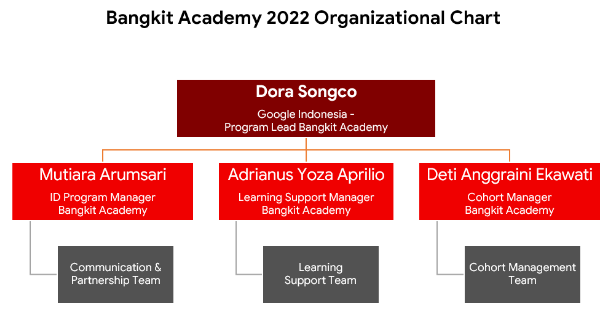
\includegraphics[width=\textwidth]{chapters/images/bangkit-2022-org-diagram.png}
    \caption{\textit{Bangkit Academy 2022 Organizational Chart}}
    \label{fig:gambar3.1}
\end{figure}

\section{Lingkup Pekerjaan} \label{lingkup-pekerjaan}

Bagian \textit{learning path cloud computing}, yaitu \textit{path} yang saya pribadi ambil dalam program ini membahas mengenai utilisasi dari \textit{cloud}, secara esensinya adalah \textit{server} yang dapat diakses oleh internet yang dibagi menjadi dua bagian besar \textit{private} dan \textit{publik}, secara spesifiknya dalam program ini, siswa \textit{cloud computing} diharapkan dapat menggunakan \textit{cloud platform} milik \textbf{Google} yaitu \textbf{GCP} atau \textbf{Google Cloud Platform}, serta memahami hal-hal teknis yang perlu diketahui untuk menggunakan \textit{cloud platform} secara efektif.

Melihat proyek yang telah dilakukan, hal ini berkaitan mengenai \textit{infrastructure} dan \textit{architecture planning}, yang dilakukan pada saat tahap \textit{pre-working} dalam proyek. Pengintegrasian \textit{services} pada tahap pengerjaan, serta pada akhirnya mendapatkan aplikasi yang bekerja secara sepenuhnya pada tahap \textit{post-working}.

\section{Deskripsi Pekerjaan}

Masuk ke topik lingkup yang sudah dibahas secara sekilas pada \ref{lingkup} kegiatan dalam program baik dalam program yang saya jalani; \textit{cloud computing}, serta \textit{learning path} lainnya (dengan perbedaan material dan \textit{provider} pada \textit{self-paced course}), terdiri dari empat kategori besar, dengan tiga dari empat kegiatan yang dimaksud bersifat wajib dan satu kategori kegiatan tidak bersifat wajib.
\begin{itemize}
    \item \textit{Self-paced Courses}: Yang terdiri dari kursus yang diambil dari tiga \textit{provider} (\textbf{Dicoding}, \textbf{Coursera} dan \textbf{Qwiklabs}), setiap kursus memiliki materi yang perlu dipelajari oleh siswa dengan tenggat waktu yang sudah ditentukan.
    \item \textit{Technical dan Soft-Skill Intructor Led Training / ILT}: Adalah pelatihan yang bekerja sebagai pengantar untuk \textit{self-paced course} (untuk \textit{ILT Tech}) dan sebagai pelatihan untuk keahlian \textit{soft-skill} (di dalamnya termasuk Bahasa Inggris), dipimpin oleh seorang instruktur yang memiliki pengalaman dalam bidangnya dan memiliki tugas pada setiap akhir \textit{ILT}.
    \item \textit{Capstone Project}: Sebuah proyek akhir yang dimana setiap peserta menggunakan keterampilan yang didapat dari program untuk membuat sebuah aplikasi dengan tema tertentu.
    \item \textit{Challenges, Guest Speakers} dan konsultasi: Sebuah tantangan yang berkaitan dengan keterampilan spesifik \textit{soft-skill} dan sesi \textit{guest speaker} dengan materi yang bervariasi. Kedua kegiatan yang disebutkan adalah \textbf{opsional}.
\end{itemize}
Setiap \textit{learning path} memiliki seluruh kegiatan yang disebutkan di atas (minus \textit{provider} tertentu dalam \textit{self-paced course}, dan diharapkan dapat menyelesaikan kegiatan-kegiatan di atas berdasarkan waktu yang telah ditentukan dalam jadwal diikuti dengan nilai yang cukup. Khusus untuk \textit{ILT}, yang wajib diikuti oleh seluruh \textit{cohort} atau siswa dalam program ini hanya dapat diikuti dengan waktu tertentu yang sudah diberikan. Siswa hanya sebatas memiliki kewajiban \textbf{menghadiri} dan \textbf{menyelesaikan tugas} yang diberikan.

\section{Jadwal Kerja}

Jadwal pada program \textbf{Bangkit 2022} memiliki acuan yang telah ditetapkan dari pihak managemen yang dapat di akses oleh seluruh anggota organisasi (siswa, dan pengurus). Jadwal pembelajaran aktif mulai dari pukul \textbf{09.00-21.00}, yang memuat rentang waktu di mana \textit{team meeting, ILT}, dan konsultasi dapat dilakukan, dan jadwal pasif (jadwal di mana siswa dapat melakukan aktivitas kursus) sepenuhnya diatur oleh siswa.

Sedangkan jadwal keseluruhan yang memuat \textit{rundown} topik yang akan dibahas pada kursus, dan \textit{ILT} dapat dibagi menjadi 5 tahap, dengan 3 tahap awal ditentukan dengan \textit{milestone} yang memiliki rentang satu sampai paling banyak empat minggu, dan dua sisanya merupakan tahap \textit{capstone} dan \textit{post-capstone}, dengan ringkasan sebagai berikut:

\begin{enumerate}
    \item Milestone 1: \textit{Web development} dan \textit{JavaScript}
    \item[] 7 Februari 2022 - 7 Maret 2022, membahas mengenai pengembangan web dan bahasa pemrograman \textit{JavaScript}.
    \begin{itemize}
        \item 4 ILT (2 \textit{tech}, 1 soft-skill, 1 english).
        \item Dua buah kursus yang berkaitan dengan topik.
        \item Satu tugas soft-skill.
    \end{itemize}
    \item Milestone 2: \textit{Backend development} dan \textbf{GCP}
    \item[] 14 Maret 2022 - 28 Maret 2022. membahas mengenai pengembangan web lebih tepatnya \textit{Backend} dan pengenalan pada \textbf{GCP}.
    \begin{itemize}
        \item 3 ILT ( 2 soft-skill, dan satu \textit{tech}).
        \item 3 buah kursus yang berkaitan dengan topik.
        \item Satu tugas soft-skill.
    \end{itemize}
    \item Milestone 3: \textit{GCP}
    \item[] 4 April 2022 - 25 April 2022, membahas lebih lanjut mengenai \textbf{GCP}.
    \begin{itemize}
        \item 5 ILT (2 \textit{tech}, 2 soft-skill, satu english.
        \item 3 buah kursus yang berkaitan dengan topik.
        \item Dua buah tugas soft-skill.
    \end{itemize}
    \item \textit{Capstone Project}
    \item[] 9 May 2022 - 13 Juni 2022, mengerjakan proyek akhir.
    \item \textit{Post-capstone}
    \item[] Persiapan sertifikasi \textit{Google associate cloud engineer}, dan materi soft-skill tambahan.
    \begin{itemize}
        \item 3 ILT (satu\textit{tech}, dua soft-skill).
        \item Satu kursus.
        \item Dua tugas softkill
    \end{itemize}
\end{enumerate}

\chapter{CLOUD COMPUTING LEARNING PATH}
\section{\textit{Leveraging Cloud Computing} Dalam Kota Pintar}

Tidak menjadikan materi yang diajarkan sebagai acuan, namun secara murni hanya menjadikan proyek akhir dari program \textbf{Bangkit 2022} sebagai topik persoalan yang akan dibahas pada bagian ini, mengingat seluruh materi dan ilmu yang dipelajari memiliki kulminasi pada proyek akhir.

\subsection{Kriminalitas dan COVID-19}

Pernyataan masalah dimulai dengan peningkatan kasus kejahatan jalanan pada beberapa daerah di Indonesia \citep{IncreaseCrimeUnoff}, namun perlu dicatat bahwa peningkatan ini tidak merata karena beragam variabel yang bermain di dalamnya \citep{indonesiaCrimeInconclusive}. Inkonklusifitas tersebut semakin terlihat ketika melihat kondisi negara lain contohnya saja Amerika yang mengalami penurunan yang cukup drastis \citep{CovidAndCrime}.

Apa pun hasil analisanya, satu yang dapat disepakati adalah kasus kriminalitas dapat terjadi kapan pun dan di mana pun. Topik utama yang menjadi fokus persoalan adalah maraknya kasus \textit{street crime} yang sering terjadi saat pandemi COVID-19 meraja lela, khususnya pada ibu kota Indonesia Jakarta. Ketika pandemi tidak ada kesulitan untuk mencari tajuk berita pembegalan, perampasan, penodongan, dan lain-lain. Menyadarkan kita bahwa hal-hal seperti itu dapat terjadi kapan pun ketika seseorang sedang bepergian dari rumah ke tempat kerja, atau tempat lainnya.

Pernyataan di atas merupakan salah satu masalah yang cukup menarik untuk dihadapi, adakah suatu cara untuk mengintegrasikan suatu layanan yang ditenagai oleh komunitas suatu kota dan dibantu dengan data yang telah dimiliki oleh kota tersebut untuk mengatasi masalah ini. Keuntungan yang didapatkan memiliki potensial besar untuk merubah hidup masyarakat kota, untuk bepergian secara aman dan juga nyaman.

\subsection{Proses}

Untuk merancang sebuah solusi yang cukup \textit{feasible}, perlu dilakukan analisa mengenai fitur yang akan dikembangkan yang pada akhirnya dapat mewujudkan tujuan yang diharapkan. Mengambil inspirasi dari digitalisasi sistem kesehatan, yaitu adanya unsur "reaktif" dan juga "preventif", aplikasi akan mendasari fungsi utamanya dengan dua istilah di atas.

\begin{itemize}
    \item Reaktif
    \item[] Mengacu kepada sistem \textit{countermeasure}, atau apa yang harus dilakukan oleh aplikasi jika terjadi tindak kriminalitas yang dialami pengguna. Hal ini memang cukup terbatas dimulai dari, akses data yang dimiliki oleh aplikasi. Karena aplikasi tidak memiliki "mata" dan "telinga" namun memiliki pengetahuan posisi di mana pengguna berada, maka fitur reaktif ini dapat dimplementasikan ke dalam sistem yang akan mendeteksi jika seseorang keluar dari kebiasaan atau lokasi yang sering dikunjungi (dengan \textit{triage} tentunya).
    \item Preventif
    \item[] Mengacu kepada sistem atau layanan yang dapat diberikan kepada pengguna untuk memberikan informasi bersih yang sudah diolah, untuk mengidentifikasi daerah yang berbahaya, diikuti dengan fitur pemilihan rute (yang akan digunakan jika pengguna akan melakukan perjalanan dari poin a ke b) yang memiliki algoritma khusus yang akan memilih rute berdasarkan hasil analisa di tahap pertama.
\end{itemize}

Perlu dijelaskan bahwa pendefisian (kami) mengenai preventif adalah sebuah cara atau sistem yang dapat memberitahu pengguna sebelumnya terhadap kondisi yang terfokus pada jumlah, tipe, dan keseringan kasus kriminalitas yang ada. Sedangkan reaktif, merupakan sebuah \textit{countermeasure} yang akan dilakukan jika sistem preventif gagal melindungi.

Dari kedua gambaran di atas dapat tergambar sedikit mengenai arsitektur sistem dan aplikasi yang akan dibuat, beserta data yang sekiranya dibutuhkan. Untuk mengimplementasi sistem preventif, diperlukan sebuah data yang memuat batasan kecamatan dari daerah yang akan digunakan untuk uji coba (dalam hal ini Jakarta), statistik kasus kriminalitas yang terjadi di daerah yang bersangkutan dan sebuah sistem \textit{routing} guna membuat sistem \textit{routing} preventif yang dimaksud.

Kemudian penentuan lingkup, menganalisa hal hal tadi untuk mengembangkan solusi reaktif pada seluruh wilayah yang ada di indonesia, hampir mustahil dilakukan dengan sumber yang sangat terbatas, sehingga pemilihan lingkup menjadi salah satu faktor penting. Jika ruang lingkup yang terlalu kecil dapat menyebabkan hasil analisa terlalu bias karena hanya didasari dengan data yang terbatas, dan juga pada akhirnya tidak berguna karena pengguna yang dapat merasakan manfaat sistem hanya akan dirasakan pada zona yang cukup kecil. Namun, jika terlalu besar, data geografis dan analisa yang perlu dilakukan sangat-amat besar jumlahnya, sehingga mengutip pernyataan sebelumnya lagi-lagi akan sangat-amat sulit dilakukan dengan sumber daya yang sangat terbatas.

Data statistik merupakan sebuah masalah yang cukup sulit dihadapi, mengingat berdasarkan data \textit{BPS} yang berupa total kasus kriminalitas tidak memberikan lokasi persis terjadinya sebuah kejahatan (patut dimaklumi karena hal ini dirasa cukup sensitif) dan melihat data tingkat kriminalitas luar hal ini juga merupakan masalah. \textbf{Data komprehensif mengenai jumlah kejahatan, lokasi terjadi berdasarkan distrik, diikuti dengan jenis kejahatan cukup mudah ditemukan}, yang menjadi masalah utamanya adalah persebaran \textit{exact} kejahatan tersebut (yang berbentuk \textit{latitude, longitude}), sehingga untuk menyebarkannya perlu dilakukan simulasi yang tidak mencerminkan keadaan sebenarnya (yang juga menjadi \textit{concern} utama tim).

Lalu pembuatan algoritma khusus yang turut terhadap data analisa nantinya pula cukup sulit dilakukan, mengingat hanya ada dua cara untuk melakukannya membuat sebuah \textit{routing system} dari nol, yang di mana hal ini adalah tugas yang cukup monumental pengerjaannya atau opsi lain yang jauh lebih memungkinkan adalah memodifikasi konfigurasi dari \textit{routing system} yang sudah ada.

Terakhir adalah pengimplementasian sistem reaktif, tim memutuskan bahwa implementasi yang paling mungkin diambil adalah sebuah \textit{habit tracker}. Dengan memanfaatkan \textit{machine learning} untuk memperkirakan rute yang biasa diambil oleh pengguna dan juga meramal posisi selanjutnya dari pengguna. Hal ini memunculkan beberapa masalah yang cukup sulit dihadapi mulai dari:
\begin{enumerate}
    \item Keamanan data pengguna, karena data yang dihadapi dirasa cukup sensitif dan akan memiliki dampak kepada pengguna jika adanya kebocoran data tanpa adanya sistem enkripsi.
    \item Arsitektur model yang berada pada tingkat lanjut, harus dapat menyesuaikan dengan kebiasaan masing-masing individu yang sangat berbeda pola-nya.
\end{enumerate}

\subsection{Perancangan Solusi}

Mendasarkan solusi berdasarkan subbab di atas, yang jika disimpulkan memiliki dua fitur utama, fitur preventif yang terdiri dari dua fitur utama \textit{overview} statistik kriminalitas yang akan diolah dengan \textit{clustering machine learning} yang diharapkan dapat mendeteksi \textbf{crime hotspot}\citep{CrimeHotspotsNIJ} yang ada dalam ruang lingkup kota yang digunakan. Sistem \textit{routing} yang akan mengkomplemen performa kerja sistem preventif, yang akan secara aktif bekerja merekomendasikan rute teraman yang dapat diambil oleh pengguna dan terakhir sistem preventif yang hanya terdiri dari satu fitur, yaitu \textit{habit tracking}.

\subsection{Safe Route}

Sebuah hasil dari perancangan solusi pencegahan kriminalitas secara \textit{preventive} dan \textit{reactive}, dengan memanfaatkan tiga fitur utama yang dapat mengkomplemen satu sama lain untuk mencapai satu tujuan yang diharapkan, dapat bekerja sebagai pencegahan dan \textit{countermeasure} jika hal kasus kriminalitas benar terjadi terhadap individu yang menggunakan aplikasi ini, dan bekerja sebagai layanan yang dapat memperkuat kualitas hidup dalam perkotaan dengan sistem preventifnya yang ditenagai oleh komunitas itu sendiri.

Sesuai dengan perancangan solusi yang telah dijabarkan pada subbab sebelum-sebelumnya, implementasi yang didapat adalah berupa aplikasi Android yang ditenagai dengan komponen \textit{backend} pendukung melewati \textbf{Google Cloud Platform} dan komponen kecerdasan artifisial yang diimplementasikan dengan \textbf{scikit learn} dan \textbf{TensorFlow}. Detail komprehensif adalah sebagai berikut:
\begin{enumerate}
    \item Sistem \textit{overview statistik} dengan \textit{overlay} yang disediakan oleh \textbf{Google Maps}, dan data \textbf{Open Street Maps Jakarta} untuk memberikan \textit{overlay} kecamatan.
    \item Sistem \textit{routing} yang untuk sementara digantikan dengan sistem navugasi \textbf{Google Maps}, karena adanya kendala dalam melakukan pengaturan server untuk menyesuaikan dengan \textit{geofence} yang telah dihasilkan.
    \item Sistem pendukung \textit{clustering} yang dilakukan sebagai \textit{job} pada proses \textit{ETL Pipeline}, yang hasil transformasi datanya digunakan pada fitur \\textit{overview} statistik. Serta pengimplementasian \textit{habit tracker} dengan \textit{TensorFlow} dengan kapabilitas terbatas.
\end{enumerate}
Hasil akhir sudah dapat digunakan, namun masih ada rasa ragu karena penyebaran data yang masih dilakukan secara artifisial, untuk langkah selanjutnya yang dapat diambil dapat dilakukan dengan terlebih dahulu melakukan riset terhadap penyebaran kasus kriminalitas di Indonesia, dan lalu dapat dilakukan \textit{pilot testing} pada kota Jakarta dengan sedikit perubahan pada sistem dan aplikasi.

\section{Pengembangan Safe Route}

Mengacu kepada deskripsi pekerjaan, serta subbab di atas, yang bertujuan untuk mengaitkan ilmu yang didapat disertai dengan pernyataan yang ada. Pelaksaan pengembangan dapat dibagi menjadi 3 bagian besar.
\begin{enumerate}
    \item Tahap pre-\textit{development}
    \item Tahap pengembangan atau \textit{development}
    \item Tahap post-\textit{development}
\end{enumerate}

 \subsection{\textit{Pre-development}}
 
\textit{Pre-development} dimulai dari membuat gambaran kasar dari aplikasi yang akan dibuat, konsiderasi dari fitur-fitur utama dan pendesignasian peran fitur utama tadi. Pendesainan antarmuka aplikasi, diikuti dengan pengembangan perangkat yang akan digunakan dalam pengembangan (dalam kasus kami sebuah website), serta menginisiasi proyek dengan menetapkan jadwal proyek, penentuan \textit{framework agile} yang digunakan, dan pada akhirnya \textit{kickoff meeting}, yang bertujuan untuk secara resmi memulai proyek.

Pelacakan kemajuan dilaksanakan lewat \textit{platform} \textbf{GitLab} yang memuat tabel \textit{kanban} yang akan menjadi patokan umum kemajuan proyek dan juga sebagai media visibilitas antar tim.

Prosedur pengerjaan juga diatur pada tahap ini yang di mana kami sepakat untuk melaksanakan \textit{daily meetup} untuk memitigasi terjadinya kesalah pahaman dan juga agar hasil pengerjaan terfokus.

\subsubsection{\textit{Development}}

Tahap pengembangan dimulai secara pararel, setiap \textit{learning path} langsung melakukan tugasnya masih-masing pada tahap awal, memulai pengembangan \textit{proof of concept} dari aplikasi yang akan digunakan dan pengumpulan (serta generasi) data. Tim \textbf{Android} melakukan pengembangan purwarupa dengan implementasi \textbf{Google Maps} pada laman utama aplikasi, disertai dengan pembuatan desain antarmuka. Tim \textit{cloud computing} melakukan pengembangan sistem autentikasi dengan \textbf{JWT}, situs web untuk purwarupa sistem, dan situs web marketing. Tim \textit{machine learning} melakukan pengumpulan data dan generasi data berdasarkan data yang telah diambil dan lalu melakukan \textit{clustering} untuk membuat model yang akan digunakan dalam \textit{ETL pipeline} pada sistem preventif.

Tahap pengembangan awal ditandai dengan terwujudnya sistem reaktif \textit{overview} statistik, tidak ada masalah yang berarti untuk tahap awal. Tahap selanjutnya adalah tahap pelaksanaan routing, pada tahap ini terjadi masalah yang di mana \textit{routing engine} yang rencananya akan digunakan, hanya mendukung subversi rute berdasarkan \textit{polygon} tidak dapat (atau kami tidak tahu cara menyesuaikannya) agar bisa melakukan subversi dari radius \textit{geofence}. Sesuai dengan dokumen \textit{risk management} yang telah dibuat pada tahap \textit{pre-development} kami memutuskan untuk menggunakan sistem navigasi \textbf{Google Maps} untuk sementara. Selain itu pelaksanaan \textit{deployment} untuk fitur statistik dilakukan dalam \textbf{GCP}, penginisialisasian database, \textit{ETL pipeline}, dan komponen \textit{backend}. Sedangkan tim \textit{machine learning} melakukan riset untuk pembuatan fitur terakhir \textit{habit tracking}.

Tahap pengembangan akhir sebelum tahap penyempurnaan adalah, \textit{habit tracker} banyak masalah yang dihadapi oleh tim pada tahap ini, mulai dari sistem \textit{parsing} yang tidak bekerja pada \textit{container} inferensi model \textit{habit tracker}, masalah pada \textit{broadcast} notifikasi daerah berbahaya yang dikaitkan dengan area yang berada dalam \textit{geofence}, komponen \textit{backend} yang tidak stabil, dan konsumsi data yang tidak dapat dilakukan oleh model yang telah dibuat. Berikut adalah langkah yang diambil untuk mengatasi masalah-masalah di atas:
\begin{enumerate}
    \item Masalah pada model \textit{habit tracker}, diselesaikan dengan implementasi manual menggunakan \textit{container} dan server web yang dibuat sendiri oleh tim, sehingga memberikan kebebasan dalam menentukan bagaimana data akan dikonsumsi oleh model untuk melakukan prediksi.
    \item Pembuatan \textit{endpoint} alternatif untuk komponen \textit{backend} yang tidak stabil.
    \item Sayangnya masih ada masalah pada sistem \textit{broadcast notifikasi}, sehingga mau tidak mau harus menerima kondisi ini.
\end{enumerate}

\subsection{\textit{Post-development}}

Tahap pasca pengembangan dimulai dengan merapihkan dokumen kerja, pembuatan presentasi dan video yang akan menunjukkan aplikasi \textbf{Safe Route}. Setelah penilaian project dapat dikerjakan lagi jika tim berkenan.

\section{Hasil Pengembangan Safe Route}

Pengembangan aplikasi (beserta subkomponenya) yang memiliki tujuan utama untuk membuat kota-kota di Indonesia lebih aman dengan bantuan komunitas sehingga diharapkan angka kasus kriminalitas.

Aplikasi ini terdiri dari tiga komponen besar yang merefleksikan masing-masing \textit{learning path} \textbf{Bangkit 2022}, selain keberhasilan pengembangan aplikasi jadi, pengembangan komponen \textit{cloud} yang mencakup \textit{backend, infrastruktur, database} dan web, pengembangan komponen \textit{machine learning} yang mendesain model secara keseluruhan.

\chapter{PENUTUP}
Pembelajaran dalam program \textbf{Bangkit 2022} dirasa cukup untuk dapat membantu mengatasi krisis talenta digital yang sedang dihadapi Indonesia, dibuktikan dengan materi yang komprehensif pada tiap \textit{learning path}, dan keberhasilan pada pengembangan aplikasi proyek akhir yaitu \textbf{Safe Route} yang menjadi testimoni kualitas program dan sebagai proyek yang menjadi \textit{highlight} dari laporan ini yang berperan sebagai sebuah aplikasi disertai dengan sistem yang diharapkan dapat mengurangi tingkat kriminalitas di Indonesia khusunya di kota-kota besar.

\section{Kesimpulan}

Program \textbf{Bangkit 2022} memiliki materi yang cukup komphrehensif untuk masing-masing \textit{path}, diikuti dengan pengembangan karakter siswanya. Pembelajaran yang meliputi:
\begin{itemize}
    \item Pengembangan Web
    \item \textit{Cloud Computing Platform}
\end{itemize}
Yang kemudian diimplementasikan langsung ke dalam proyek akhir (\textit{capstone project} menjadi testimoni kualitas program. Sedangkan bila proyek akhir disimpulkan akan diperoleh poin-poin sebagai berikut:
\begin{itemize}
    \item Berhasilnya pengembangan aplikasi \textbf{Safe Route} dengan kolaborasi dari ketiga unsur \textit{learning path} yang ada di \textbf{Bangkit 2022}.
    \item Sistem eksperimental pencegahan kriminalitas secara preventif dan reaktif yang ditenagai kecerdasan artifisial dan \textit{cloud computing platform \textbf{GCP}}.
    \item Aplikasi yang dibuat secara \textit{native} dengan \textbf{Kotlin}.
\end{itemize}

\section{Saran}

Terdapat beberapa hal yang dapat diperbaiki dalam rangka membantu dan mengembangkan kemajuan program ke depannya hal ini adalah:
\begin{itemize}
    \item Ilmu komputer dasar yang mencakup jaringan, sistem operasi, dan Linux dirasa perlu dilakukan.
    \item Transparansi sistem penilaian.
    \item Perbaikan beberapa sistem seperti absensi dan sistem \textit{feedback} yang kurang maksimal.
    \item Ketepatan waktu jadwal, terjadi banyak keterlambatan di akhir.
\end{itemize}
Sedangkan bila berbicara mengenai proyek akhir yang dikerjakan, yaitu \textbf{Safe Route} berikut adalah saran-saran yang ditunjukkan kepada siapapun yang ingin ikut menyempurnakan aplikasi serta sistemnya:
\begin{itemize}
    \item \textit{Business model} perlu diperkuat, karena pada fase yang ada sekarang tidak banyak kesempatan untuk mendapatkan keuntungan.
    \item \textit{ETL pipeline(s)} yang lebih matang.
    \item Serta data riil yang dapat merefleksikan kejadian kejahatan secara akurat.
\end{itemize}


% \chapter{KESIMPULAN DAN SARAN}
% Bab ini menyatakan pemahaman peneliti tentang masalah yang diteliti berkaitan dengan tesis/disertasi berupa simpulan dan saran.

\section{Simpulan}
Sub-bab ini menyatakan temuan-temuan penelitian berdasarkan hasil penelitian dan pembahasan.

\section{Saran}
Sub-bab ini menyatakan saran teoretis tentang apa yang perlu diteliti lebih lanjut untuk pengembangan ilmu pengetahuan dari bidang ilmu yang dikaji, serta saran praktis yang terkait dengan penyataan penerapan ilmu pengetahuan terkait.

Bila bagian hasil dan pembahasan disajikan dalam lebih dari 1 (satu) bab, maka penomoran bab simpulan dan saran disesuaikan dengan jumlah bab yang ditulis sebelumnya (bab simpulan dan saran adalah bab terakhir dari Tesis/Disertasi).


%%%%%%%%%-----DAFTAR PUSTAKA-------%%%%%%%%%%%%%%%%%%%%%%%%%%%%%%%%%%%%%%%%%%%%%
\singlespacing
\bibliographystyle{plain} %% modifikasi gaya sitasi dari dcu
\renewcommand{\bibname}{Referensi} % ubah "bibliography" menjadi "Daftar Pustaka"
\newpage
\setcounter{page}{9}
\renewcommand{\thepage}{\roman{page}}
\bibliography{contoh_pustaka}

\newpage
\setcounter{page}{1}
\renewcommand{\thepage}{A-\arabic{page}}
\addcontentsline{toc}{chapter}{Lampiran A (TOR)}

\chapter*{Lampiran A (TOR)}
{\setstretch{1.5}

\section*{Completions Requirements (Bangkit Welcome Kit)}

Careful planning has gone into designing the curriculum for this program from beginning to end. At the conclusion of the program, all participants who meet the completion criteria, will be regarded as Bangkit Graduates and given certificate of accomplishment/completion and a complete transcript. Those who didn’t complete all the Bangkit will get Certificate of Attendance and partial transcript. Bangkit Graduates will also receive a voucher for the certification exam of their respective Learning Path. The requirements for graduation from Bangkit 2022 are as follows:


\begin{itemize}
    \item \textbf{Attending and actively participating in mandatory sessions,} including but not limited to:
        \begin{itemize}
            \item Bangkit 2022 Opening Session
            \item 80\% of the Instructor-led sessions for Tech* 
            \item 80\% of the Instructor-led sessions for Soft Skills*
            \item 90\% of mandatory guest/special lectures*
        \end{itemize}
    \item[] \textbf{Sessions will be informed at least 7 calendar days before. So please check your calendar on a daily basis}
    \item \textbf{For self-paced sessions, you just need to complete them in the same week.}
    \item[]If you have things to do for the allocated self-paced time, you don’t need to fill the form. Just allocate another time outside Bangkit allocated time to study and adjust by yourself. As you’re aware, the Bangkit learning method combines online self-paced study, online synchronous / instructor-led training (ILT), and project-based learning. Therefore, to help you plan your time, we have created a Bangkit learning schedule.
    \item \textbf{Submit your own work for assignments and projects.}
    \item[] Bangkit is part of the Kampus Merdeka program where academic honesty is upheld. You should demonstrate and uphold the highest integrity and honesty in all the academic work that you do. Plagiarism isn’t permitted and score for the respective assignment will be void/canceled in the event your work is flagged for plagiarism. Our learning platform partners may ban or disable your account if you plagiarize or are dishonest based on their sole discretion.
    \item \textbf{Completing official Bangkit assignments} (including classroom and our learning platform partners - Dicoding, Google Cloud Skills Boost, Coursera) each in accordance with their respective standards. Late submission will be accepted, but will reduce the respective assignment score.
    \item \textbf{Contributing to Bangkit Capstone Project.}
    \item[] This will be scored by the Bangkit Committee and your team members and includes your attendance in the final project presentation. 
    \item \textbf{Adhering to the Bangkit Code of Conduct}
\end{itemize}
}


\newpage
\setcounter{page}{1}
\renewcommand{\thepage}{B-\arabic{page}}
\addcontentsline{toc}{chapter}{Lampiran B Log Activity}

\chapter*{Lampiran B (Activity Log)}
\section*{\textit{Activity Log}}

\setstretch{1.5}
Bagian ini membahas secara detil kegiatan yang dilakukan pada saat program berlangsung. Kegiatan tentunya berdasar dari penjelasan yang telah diberikan sebelumnya. Tabel digunakan sebagai preferensi struktur \textit{activity log}, disesuaikan dengan format yang telah diberikan sebelumnya. Log tidak dibagi berdasarkan kegiatan per hari yang dilakukan namun dengan rentang seminggu yang direferensikan ke dalam jadwal resmi yang sudah dikeluarkan oleh pihak \textit{Bangkit 2022}, kolom kegiatan memuat seluruh kegiatan yang dilakukan pada rentang waktu tersebut dengan \textit{mention} kegiatan dan tidak akan membahas apa yang kegiatan tersebut bahas, tugas tertentu dalam kegiatan maupun materi yang dibahas oleh kegiatan tersebut.


\setstretch{1.5}
Hasil merupakan seperti namanya menandakan hasil yang didapat dari kegiatan yang dilakukan, hal ini dapat berupa tugas yang perlu diselesaikan atau sudah diselesaikan, proyek akhir kegiatan, maupun sertifikasi yang didapat oleh peserta. Di halaman berikutnya akan memuat tabel yang dimaksud, terdiri dari tabel-tabel yang merangkum secara singkat namun komphrehensif.


\begin{tabular}{ |p{3cm}|p{6cm}|p{3cm}|  }
 \hline
 \multicolumn{3}{|c|}{Log Kegiatan} \\
 \hline
 Minggu/Tanggal & Kegiatan & Hasil\\
 \hline
 0/7 Februari & Matrikulasi, dan kegiatan \textit{prework} & \textbf{GCP intro}, gitlab usage, \textit{programming intro} \\
 \hline
 1/14 Februari & Kursus \textit{Basic web development} di Dicoding & \textit{Static web} \\
 \hline
 2/21 Februari & \textit{Pre-read} ILT \textit{Time management}, akhir \textit{Basic web development}, mulai kursus, ILT Tech 1 \textit{JavaScript Basic} & Proyek web statis, sertifikat \textit{Basic Web Development Dicoding} \\
 \hline
 3/28 Februari & ILT \textit{Time management}, Kursus \textit{JavaScript Basic} & Essay pada \textit{time management} \\
 \hline
 4/7 Maret & Tugas \textit{time management}, ILT \textit{English Spoken Correspondence}, \textit{Pre-read Professional Branding} Akhir kursus \textit{JavaScript}, awal \textit{Backend Basic}, ILT Tech 2 & Pengumpulan tugas \textit{time management}, nilai ujian akhir kursus JavaScript disertai sertifikat dan \textit{quiz english spoken correspondence} \\
 \hline
\end{tabular}


\begin{tabular}{ |p{3cm}|p{6cm}|p{3cm}|  }
 \hline
 \multicolumn{3}{|c|}{Log Kegiatan} \\
 \hline
5/14 Maret & ILT \textit{Professional Branding \& Interview}, Akhir kursus \textit{Backend Basic}, awal kursus lab \textit{Google Cloud Computing Fundamentals} & \textit{Bookshelf API} disertai sertifikat, \textit{resume proper writings} \\
 \hline
 6/21 Maret & Tugas \textit{Professional Branding \& Interview}, \textit{Pre-read Critical Thingking}, \textit{Google Cloud Computing Fundamentals}, ILT Tech 3 & Essai \textit{Professional Branding \& interview}, \textbf{Qwiklabs badges} dan GCP \textit{stuffs} \\
 \hline
 7/28 Maret & ILT \textit{Critical Thingking}, \textbf{Qwiklab Quests} \textit{(Developer essentials, DevOps, Interactive apps, website}, awal kursus \textbf{Coursera} \textit{Architecting with Google Cloud Engine} & \textbf{Qwiklabs badges} dan sertifikat course 1 kursus \textit{Architecting with Cloud Engine} \\
 \hline
 8/4 April & Tugas \textit{Critical Thingking}, \textit{Pre-read Adaptability}, ILT Tech 4, Kursus 2 \textit{Architecting with Google Cloud Engine}, \textbf{Qwiklab quests} \textit{(Create and manage cloud resources, Foundational infrastructure task, Foundational Data, ML, and AI)} & Essai \textit{Critical Thingking}, Sertifikat kursus 2 \textit{(Architecting with GCE)}, \textbf{Qwiklab badges} \\
 \hline
 \end{tabular}

\begin{tabular}{ |p{3cm}|p{6cm}|p{3cm}|  }
 \hline
 \multicolumn{3}{|c|}{Log Kegiatan} \\
 \hline
 9/11 April & ILT \textit{Adaptability}, Kursus 3 dan 4 \textit{(Architecting with GCE), \textbf{Qwiklab quests} \textit{(Build and secure networks, Monitor and logs with Operations Suite)}} & Sertifikat 3 \& 4 \textit{(Arhitecting with GCE)}, \textbf{Qwiklab badges} \\
 \hline
 10/18 April & Tugas \textit{Adaptability}, \textit{Pre-read Idea Generation \7 MVP}, ILT Tech 5, Kursus 5 \textit{(Architecting with GCE)}, \textbf{Qwiklab quests} \textit{(Cloud Architecture, Understanding \& Optimizing Google Cloud Cost, Security \& Identity Fundamentals} & Sertifikat \textit{specialization (Architecting with GCE)}, \textbf{Qwiklab badges} \\
 \hline
 11/25 April & ILT \textit{Idea Generation \& Planning}, \textbf{Qwiklab quest} \textit{(Cloud Logging, Deploy to Kubernetes)}, Kursus \textbf{Coursera} \textit{Preparing for ACE Certification} & \textbf{Qwiklab badges}, Sertifikat \textit{Preparing for ACE Certification}. \\
 \hline
 12/9 May & Tugas \textit{Idea Generation \& MVP}, \textit{Capstone Project} & Essai \textit{Idea Generation \& MVP}, \textit{Safe Route Project Artifacts} \\
 \hline
\end{tabular}

\begin{tabular}{ |p{3cm}|p{6cm}|p{3cm}|  }
 \hline
 \multicolumn{3}{|c|}{Log Kegiatan} \\
  \hline
  13/16 May & ILT \textit{English Business Presentation}, \textit{Capstone Project} & \textit{Quiz English Business Presentation}, \textit{Phase 1 Safe Route Overview Statistics Development} \\
 \hline
 14/23 May & \textit{Capstone Project} & \textit{Phase 2 Safe Route, Routing System, Integrations}\\
 \hline
 15/30 May & \textit{Capstone Project} & \textit{Phase 3 Safe Route, Artificial System Development}\\
 \hline
 16/6 Juni & \textit{Capstone Project} & \textit{Final Phase, Deployments \& Polishing} \\
 \hline
 17/13 Juni & \textit{Capstone Project}, \textit{Pre-read Startup Valuation} & Finalisasi \textbf{Safe Route} \\
 \hline
 18/20 Juni & ILT \textit{Startup Valuation}, \textit{English Post-test}, awal \textbf{Dicoding} \textit{Cloud Certification simulation exam} & Tugas \textit{Startup Valuation} \\
 \hline
 19/27 Juni & \textit{Pre-read Professional Communication}, akhir \textbf{Dicoding} \textit{Cloud Certification simulation exam} & Preparasi \textbf{Google ACE} \\
 \hline
  20/4 Juli & ILT \textit{Professional Communication}, Kelas \textit{Expert} (Opsional) & Essai \textit{Professional Communication} \\
  \hline
  21/11 July & \textit{Post Program} & Program selesai \\
  \hline
\end{tabular}

\newpage
\setcounter{page}{1}
\renewcommand{\thepage}{C-\arabic{page}}
\addcontentsline{toc}{chapter}{Lampiran C Dokumen Teknik}

\chapter*{Lampiran C Dokumen Teknik}
{\setstretch{1.5}
\section*{Pratinjau}

Bagian ini memuat dokumentasi lengkap \textit{capstone project} dari \textbf{Bangkit 2022} yang diikerjakan oleh saya pribadi dengan 4 rekan saya lainnya yang terdiri dari Hanif Adam Al-Abraar (Universitas Brawijaya), Muhammad Anggi Wirahmat (Universitas Presiden), Fillah Akbar Firdausyah (Universitas Amikom Yogyakarta), Ikhsan Cahya Mardika (Universitas Gunadarma), Christopher Chandrasaputra (Institut Teknologi Bandung). \textbf{Semua dokumentasi teknis, kode sumber, serta aplikasi (fungsionalitas kemungkinan terbatas karena adanya unsur cloud computing yang menggunakan biaya) pada tautan berikut gitlab.com/safe-route}

\subsection*{Tema Pilihan}
\textit{Mobility \& Smart City}

\subsection*{Background}
\textit{Due to the recent increase in crime rate, we need to find a way to protect society from increasing crime rates, especially in larger cities. One way to do this is to create safe transportation options for people who need to commute to the city. To address this problem, we have the idea of protection, in particular those who are as vulnerable as women and children, so that they know which route is the safest, thus avoiding the emergence of potentially dangerous areas. This is useful for newcomers in cities to remind those already living in cities and to further improve the quality of life in urban areas. Based on what we've heard about crime rates in the city, we think it would be a good idea to use artificial intelligence to help people figure out which areas are especially dangerous and then provide them with directions to avoid these areas.
}

\subsection*{Implementation}
All of the implementation we did pre-working on the project includes the design of the layout in Figma, architecture overview of potentially used services in GCP, and lastly model prototype of habit tracker.
\begin{itemize}
    \item For UI design with Figma: We wanted to have a lay of the land before doing the actual app even though the app that we’ve made does not exactly follow the design that we’ve already made before.
    \item For cloud architecture we build a simple architecture that will expand following Android and Machine Learning request, for example we starting small from just  using AI Platform and Cloud API in the plan, to a full fledged many services like google cloud storage, BigQuery, Firestore, Cloud Functions, Cloud Run, and Compute Engine.
    \item In Machine Learning a simple diagram prototyping the model is done, firstly the clustering model is based on the paper mentioned above (E. Eck 2005) as a basis for clustering, and then TensorFlow as the Forecasting model.
\end{itemize}

For improvements based on the evaluation we’ve done post-project, includes some of the suggestion suggested by us from the mentors that are not fulfilled yet which includes:
\begin{itemize}
    \item The data that is used must be collected accurately, as the data we are using now is only a dummy data (the latitude and longitude is still made up but still being based on BPS statistics).
    \item Improvements on the pipelines, as the pipelines currently we have deemed to be a bit rudimentary with limited capabilities. This will improve the seamless integration of features of our application.
    \item Model architecture must be revamped too, as the current model is not ideal when scaled to a thousand of users. The use of a model that can be used to cater to the habit of each user but only use one model on the backend.
    \item Background process handling must be addressed too as currently we deemed the app to be resource consuming, a more clever way to handle background process or even a whole new flow foreign to us must be used.
\end{itemize}
}

\section*{Gambar Hasil}

\setstretch{1.5}
Berikut adalah kompilasi gambar dari implementasi yang dilakukan oleh kami, gambar diambil dari aplikasi \textbf{Safe Route} yang sedang berjalan secara langsung pada 13 Juni 2022, perbedaan aplikasi setelah tanggal tersebut dihiraukan.


\begin{figure}
    \centering
    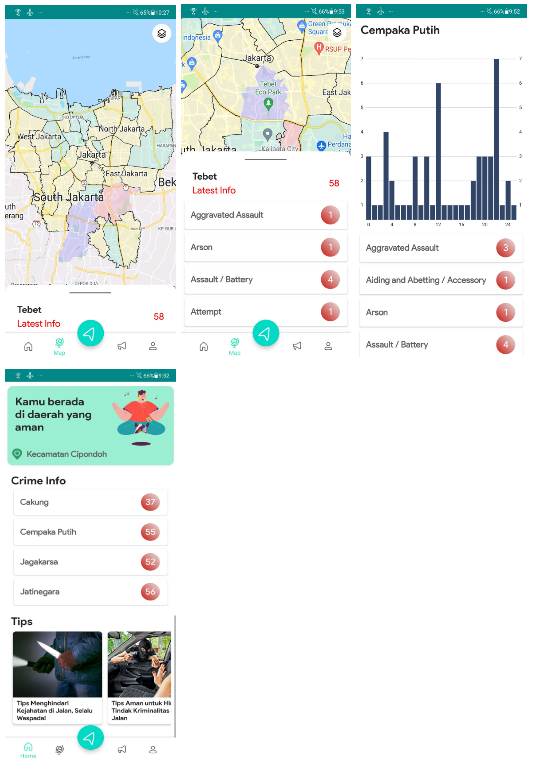
\includegraphics[width=\textwidth]{chapters/images/stats.png}
    \caption{\textit{Area statistic feature (dari kiri ke kanan) chloropleth layer, info panel, statistic drill down, overview}}
    \label{fig:gambar8.1}
\end{figure}

\begin{figure}
    \centering
    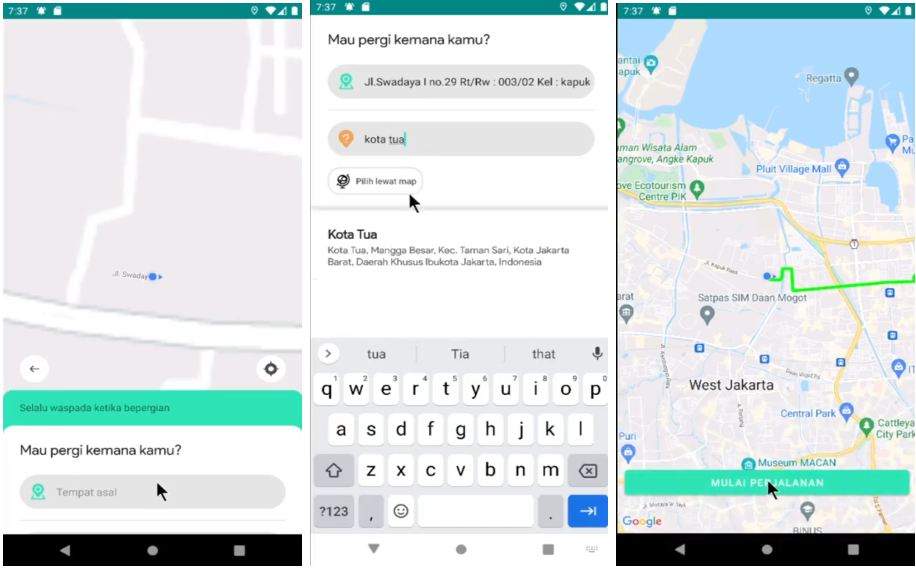
\includegraphics[width=\textwidth]{chapters/images/route-sys.png}
    \caption{\textit{Routing system in the work}}
    \label{fig:gambar8.2}
\end{figure}

\begin{figure}
    \centering
    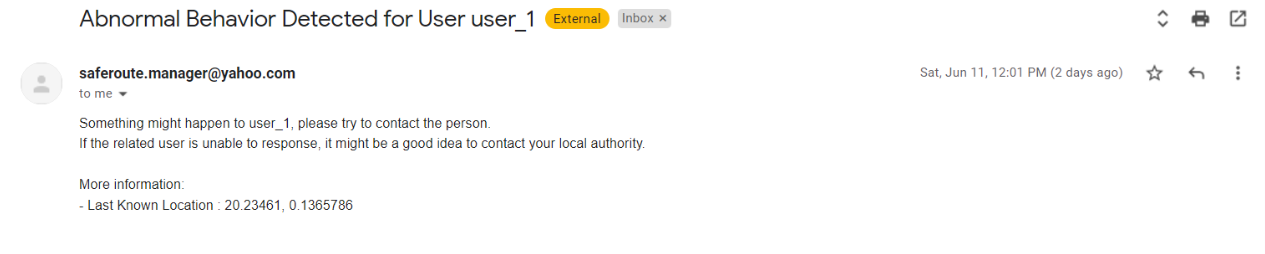
\includegraphics[width=\textwidth]{chapters/images/habit-tracker.png}
    \caption{\textit{Habit tracker anomaly respond email}}
    \label{fig:gambar8.3}
\end{figure}

\end{document}
